\documentclass[journal,twoside]{IEEEtran}
\usepackage[pdftex]{graphicx}
\graphicspath{{./microgrid/}}
\DeclareGraphicsExtensions{.pdf,.png,.jpeg}
\usepackage{amsmath}
\usepackage{array}
\usepackage{etoolbox}
\patchcmd{\thebibliography}{\section*{\refname}}{}{}{}
\patchcmd{\thebibliography}{\addcontentsline{toc}{section}{\refname}}{}{}{}
%\usepackage{url}

\begin{document}

    \setcounter{page}{18}

\title{Fully User-Compatible Microgrid Network and Its Control: A Concept}

\author{
    Sulav Ghimire\\
    Department of Electrical Engineering\\
    Institute Of Engineering(IoE), Pulchowk Campus, Pulchowk, Lalitpur\\
email: sulavggg@gmail.com\\
}

\markboth{Zerone Scholar,Vol.1, No.1, November-2016}%
{\textit{S. Ghimire}: Fully User-Compatible Microgrid Network}

\maketitle
\begin{abstract}
Microgrids have been an alternative to costly procedure of utility grid expansion to electrify a rather rural area. This paper proposes a model of microgrid with Distributed Generation (DG) and capability to interconnect with other microgrids, and also with the utility grid for power exchange, whenever necessary. The proposed structure consists of generation part, storage part, distribution part and control and conversion part. A new concept of Hybrid Energy Storage System (HESS) has been used for energy storage. Also, a fully functional control hub has been proposed, which could be used to connect number of generation units, both AC and DC, and could supply to both AC and DC distribution feeders. The scope of this proposed model is also discussed in this paper.
\end{abstract}
\begin{IEEEkeywords}
Distributed Generation, Hybrid Energy Storage System (HESS), Microgrid
\end{IEEEkeywords}

\section{Introduction}
Microgrids are isolated islanded systems which generate, manage and provide electrical energy within itself. Using microgrids, limited energy can be saved by designed source holders such as batteries but their technologies must be expertly managed to control its different aspects within the limited charge window of batteries \cite{Arnold2050}. E Becquerel created the world's first PV cell in 1839 \cite{Zamostny2013}  and in recent years, PV cells have been extensively used as Distributed Generation units in microgrids. Similarly, the use of induction generators in microhydro power plants and wind energy stations have also grown highly \cite{Liu2015}. As per the need of customers, the microgrids are either AC \cite{Liu2015} or DC \cite{Chen2015, Piagi2006, Lee2015, Madduri2015} . 
Some grids exchange with the utility grid \cite{Chen2015}  or with another microgrid \cite{Lee2015}. Such interconnections increase the reliability of the entire system. When there is low power demand on the grid (lower than generating capacity of associated generators), then it could be stored for future using HESS. Storage of generated power based on conventional storage technology using batteries only has been used previously a number of times \cite{Lee2015, Madduri2015, Vosoloo2050, Zenned2015, Latreche2015, Yahyaoui2015, Khaldi2015} . But HESS has been used only a few times \cite{Piagi2006, Lee2015, Khaldi2015}. 

\bigskip
In this paper, the proposed system is such that a central controller controls multiple AC/DC grids, enables energy exchange, energy saving and power interaction with utility grid as well. Addition of a new microgrid to that system could also be enabled. This paper is divided into seven parts, part I is introduction, part II will describe the AC units, part III will describe the DC units and the subsequent parts will be about HESS, Central controller and conclusions.

\section{AC Unit}
The proposed system has four important parts viz. ac units, dc units, HESS and Central controller. The ac unit has general structure as in Figure 1.
\begin{figure}[!ht]
\centering
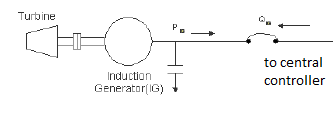
\includegraphics[width=2.5in]{1}
\caption{General Layout of ac unit}
\end{figure}
Based on the wind flow data and equipment accessibility, wind plant could be used in various places. If there is an ample water resource then micro-hydropower generation could also be used. These stations feed the energy generated directly to the controller. All further actions will be taken care of by the controller and other parts of the system. Systems similar to this structure have been used before as well \cite{Piagi2006, Liu2015, Jabri2015, Moghadam2015}.

\section{DC Units}
Wind flow governs the speed of wind turbine which in turn governs the output of the IG used. Similarly, water resource and its seasonal availability govern the power generated by micro-hydropower plant. AC generation is thus seasonal power generation technique because power generation capability depends on the season of year. So, AC grid alone is not always enough for a fully compatible microgrid architecture, neither is DC grid alone. 
\begin{figure}[!t]
\centering
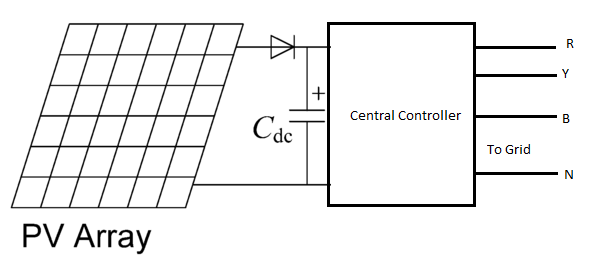
\includegraphics[width=2.5in]{2}
\caption{General Layout of dc unit}
\label{f2}
\end{figure}In order to fulfill the off season power requirements, energy storage and DC generation is also vital. In this section, DC generation will be discussed, and energy storage will be discussed in the next section. One of the best ways of dc power generation is Photovoltaic (or PV) generation system. The following structure is proposed for DC generation. PV grid generates DC power and feeds to the central controller. As before in AC generation, further actions will be handled by the controller itself. A PV structure is shown in Figure 2.


\bigskip
DC microgrids are extensively in use nowadays.
Many researchers have worked in this area such as in \cite{Chen2015, Piagi2006, Lee2015, Madduri2015, Vosoloo2050, Liu2015, Giacomini2015, Latreche2015, Yahyaoui2015}.


\section{Hybrid Energy Storage System (HESS)}
Storage of electrical energy is always a major
concern. Conventionally, electrical energy has been
stored in the form of chemical energy (batteries). But
recently, a new type of storage scheme has been
brought to use, which combines chemical storage and
storage in electric field. This technique is known as
Hybrid Energy Storage System (HESS). This system
uses batteries and super capacitors as storage units.
HESS has been proved to be highly efficient and
effective and reliable than conventional systems of
energy storage \cite{Yahyaoui2015, Ismail2013}.
State of charge (SOC) is seen as the full range
of available energy that can be delivered by a battery.
This range is measureable between when a battery is
fully charged and when it carries no charge. Because of
the limiting SOC of batteries, the problem is that the limited
energy is available for a given time. Energy management deals with controlling power flow in a system by

having a limited amount of energy, or to work with it
in a "saving manner." To extend the time of use from a
limited source, load monitoring and control are required \cite{Michaelson2050}. Hence, by analyzing the SOC of battery
used and improving the capacitor, we can improve the
HESS and its SOC.
Since Lithium-Iron-Phosphate batteries (Lipo batteries) have been proven to have longer life cycles
and higher safety in comparison to other Li-ion chemistry \cite{Lithium2050}, its use in HESS could make the storage system more effective.
The general possible schemes of HESS
structure is shown in the figure below:

\begin{figure}[!ht]
\centering
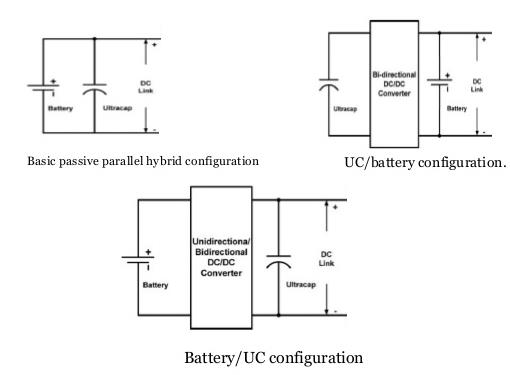
\includegraphics[width=2.5in]{3}
\caption{General Layout of HESS}
\label{f3}
\end{figure}


\section{Central Control Unit}
This unit is the heart as well as the brain of
the proposed system. In brief, the major work of this
unit is summarized below:
\begin{itemize}

\item[(i)]
To convert the voltage of a dc generating
unit to desired level and either (a) store
the power in HESS if the demand is low
or (b) invert it to AC of the provided
reference voltage for AC distribution.
\item[(ii)]
To rectify the AC from AC sources to
desired level of DC and perform action (a)
if the demand is low or (c) distribute AC
to the consumers if the demand is high.
\item[(iii)]
If the HESS is fully energized, and still
the load demand is low, this unit feds the
energy to the main grid.
\item[(iv)]
If there is energy deficiency in the
microgrid, it extracts energy from main
grid to charge the HESS or to distribute
to the consumers or do both.
\item[(v)]
If there is any fault or contingencies in
the main grid or in one or more of the
associated microgrids, central unit senses
this fault and immediately isolates the
faulty part unless the fault or anomalies has been cleared. The sensing could be
done by wavelet transform methods \cite{Moghadam2015}.

\end{itemize}


Some of the concept of this intelligent energy
management system has been used in \cite{Vosoloo2050} and some
references have been taken from the same.


\section{Simulation and Results}

A preliminary model of the proposed system
was developed in MATLABTM/Simulink 2016 and
analyzed. The overview of the model is shown in
Figure 4.
\begin{figure}[!ht]
\centering
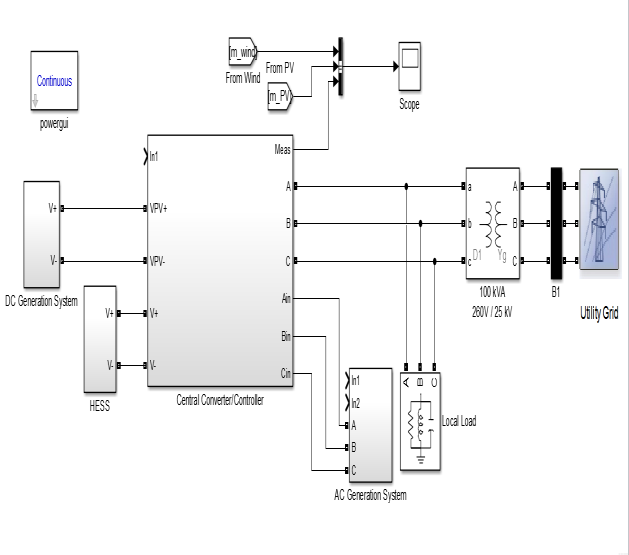
\includegraphics[width=2.5in]{4}
\caption{Outer layout of the proposed system in
Simulink}
\label{f4}
\end{figure}

The main four parts of the system in the above
picture, namely the AC generating units, the DC
generation units, the hybrid energy storage system and
finally, the central part, the central controller could be
clearly seen in Figure 4.
Taking a look at the simulated hypothetical
AC generating system of the simulation by entering the
AC subsystem, we see as below (Figure 5).

\begin{figure}[!ht]
\centering
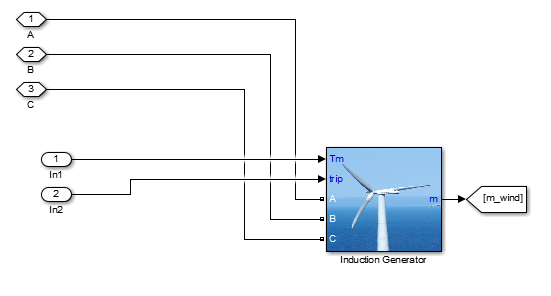
\includegraphics[width=2.5in]{5}
\caption{AC generation layouts in Simulink (Wind Energy Farm)}
\label{f5}
\end{figure}


Similarly, the DC generating unit, which is
supposed to generate DC power from PV panels, used
in this simulation is shown in Figure 6.
\begin{figure}[!ht]
\centering
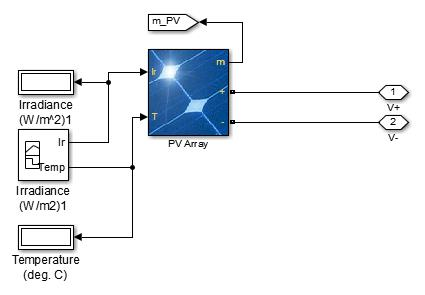
\includegraphics[width=2.5in]{6}
\caption{DC generation layouts in
Simulink(PV Solar Panels)}
\label{f6}
\end{figure}

The HESS subsystem in Figure 4 when seen
in detail looks like as in Figure 7.
\begin{figure}[!ht]
\centering
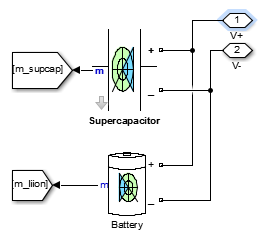
\includegraphics[width=2.5in]{7}
\caption{HESS layouts in Simulink(Battery and Supercapacittor)}
\label{f7}
\end{figure}

Finally, the most important part of the
proposed system and the simulation, the central
controller which controls all other parts and manages
ang governs the energy storage and flow is shown in
Figure 8.

\begin{figure}[!ht]
\centering
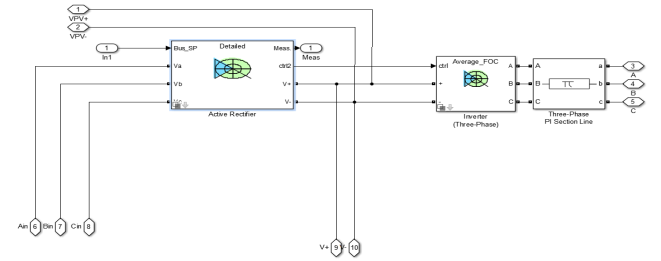
\includegraphics[width=2.5in]{8}
\caption{Scheme of the central controller in Simulink}
\label{f8}
\end{figure}
Finally, the result obtained, the
voltage profile of the grid and the DC generation units
are shown in Figure 9 and 10 respectively.

\begin{figure}[!ht]
\centering
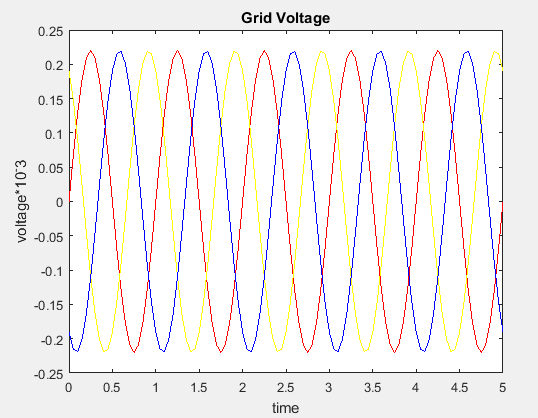
\includegraphics[width=2.5in]{9}
\caption{Utility Grid Voltage Profile}
\label{f9}
\end{figure}

\begin{figure}[!ht]
\centering
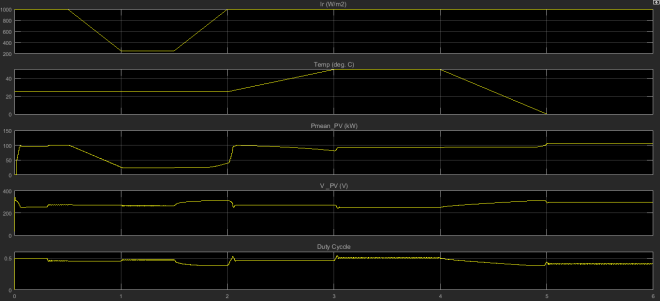
\includegraphics[width=2.5in]{10}
\caption{DC generation voltage, power and temperature and irradiance profile}
\label{f10}
\end{figure}


Remaining part of the system is under
development in MATLABTM/Simulink and the
improvement of central controller and AC generation
system is being conducted.


\section{Future Works}
The future works for the development of this system is
listed below:
\begin{itemize}
\item Improvement of the central control unit so that it
could be monitored and controlled by a
computerized system.
\item The AC generation system used in present
simulation is a very rough and preliminary work.
It needs to be upgraded and more variables should
be considered to get better results.
\item Similarly, the variables used in DC generation are
enough, but could be upgraded and new data could
be used.
\item MPPT has not been included in any of the systems.
If MPPT could be added, then the system could be
more advanced and automatic.
\item Islanding and fault detection using HF injection is
proposed to be included in the next upgrade of the
system.
\end{itemize}

\section{Conclusion}
Compared to traditional microgrids, this new
scheme involves better control of power flow, better
control over the generating units and the storage units
and provides a unique bidirectional power flow facility
from microgrid to utility grid.
Energy conversion and storage is managed by
a single unit and interconnection with utility grid is
also monitored by the same.
The generated AC power is first rectified to
DC and then further sent either to rectification for
distribution or utility grid or to HESS for storage. Apart from other advantages, AC
involves multiple rectification and inversion which
seems to be a rather lossy process. Steps are being
taken to reduce the aforementioned losses in the future
versions of this scheme.
The results presented by the developed parts
of the system, \textit i.e.\ the utility grid and the DC
generation unit look quite promising and hence show
potential for future success and development.


\section*{Bibliography}
\begin{thebibliography}{99}

    %21
    \bibitem{Arnold2050} 
        T Markvart, R Arnold, 
        \emph{Microgrid: Power Systems for the $21^{st}$ Century} 
        \lbrack Online \rbrack [Available:http://www.ingenia.org.uk/ingenia/articles.aspx?Index=329]

    %22
    \bibitem{Zamostny2013} 
        ~D Zamostny, \emph{Solar History: Alexandre Edmond
        becquerellar}, \lbrack Online\rbrack, 2 December 2013,

    %7
    \bibitem{Liu2015} 
        ~P C Liu et.al, \emph{Disturbance Rejection Strategies
        for AC/DC Microgrids}, Proceedings of the $8^{th}$ 
        IEEE GCC Conference and Exhibition, Muscat,
        Oman, February 2015

    %1
    \bibitem{Chen2015}
        ~L Chen, S Mei, \emph{An integrated control and
        protection for PV Microgrids}, CSEE Journal of
        Power and Energy Systems, Vol. 1, No. 1, March
        2015

    %2
    \bibitem{Piagi2006} 
        ~P Piagi, R H Lasseter, \emph{Autonomous Control of
        Microgrids}, IEEE 2006, ISBN: 978-1-4244-0493-2

    %3
    \bibitem{Lee2015} ~M Lee et.al, \emph{Operation Schemes of
        Interconnected DC Microgrids Through an
        Isolated Bidirectional DC-DC Converter}, IEEE
        2015, ISBN: 978-1-4799-6735-3

    %4
    \bibitem{Madduri2015} 
        ~P A Madduri et al, \emph{A Scalable DC Microgrid
        Architecture for Rural Electrification in Emerging
        Regions}, IEEE 2015, ISBN: ISBN: 978-1-4799-6735-3

    %6
    \bibitem{Vosoloo2050} 
        ~A Vosoloo, K A Raji, \emph{Intelligent Central Energy
        Management System for Remote Community
        Microgrid}, IEEE

    %13
    \bibitem{Zenned2015} 
        ~S Zenned, A Mami, \emph{Design of a Hybrid System
        for Battery Sizing to Supply a Domestic Load},
        IEEE $6^{th}$ International Renewable Energy
        Congress, 2015, ISBN: 978-1-4799-7947-9
    
    %14
    \bibitem{Latreche2015} 
        ~S Latreche, \emph{Implementation of a MPPT
        Algorithm and Supervision of a Shading on PV
        Panel}, IEEE $6^{th}$ International Renewable Energy
        Congress, 2015, ISBN: 978-1-4799-7947-9

    %15
    \bibitem{Yahyaoui2015} 
        ~I Yahyaoui et.al, \emph{MPPT Techniques for a
        Photovoltaic Pumping System}, IEEE $6^{th}$
        International Renewable Energy Congress, 2015,
        ISBN: 978-1-4799-7947-9

    %16
    \bibitem{Khaldi2015} 
        ~H S Khaldi, A C Ammari, \emph{Fractional-order
        Control of Three Level Boost DC/DC Converter
        Used in HESS for Electric Vehicles}, IEEE $6^{th}$
        International Renewable Energy Congress, 2015,
        ISBN: 978-1-4799-7947-9
    %8
    \bibitem{Jabri2015} 
        ~Y A Jabri et.al, \emph{Voltage Stability Assesment of a
        Microgrid}, Proceedings of the $8^{th}$ IEEE GCC Conference and Exhibition, Muscat, Oman,
        February 2015
    %10
    \bibitem{Moghadam2015} 
        ~M A Moghadam, et.al, \emph{ A new method for
        Islanding Detection of Distributed Generation
        Systems via Wavelet Transform based Approaches}
        The $9^{th}$ Power System Protection and Control
        Conference, IEEE 2015, Tehran, Iran
    %11
    \bibitem{Giacomini2015} 
        ~J C Giacomini et.al, \emph{Design of a LCL Filter for
        Leakage Current Reduction in Transformer-less
        PV Grid Connected Three Level Inverter}, IEEE
        2015, ISBN: 978-1-4799-6735-3
    %20
    \bibitem{Ismail2013} 
        ~M.S. Ismail, M. Moghavvemi, T.M.I. Mahlia,
        \emph{Techno-economic analysis of an optimized
        photovoltaic and diesel generator hybrid power
        system for remote houses in a topical climate},
        energy Conversion and Management 69, 163-173.
        (2013)
    %25
    \bibitem{Michaelson2050} 
        ~D Michaelson et.al, \emph{A Predictive Energy
        management Strategy with Preemptive Load-
        shedding for and Islanded PV Battery Microgrid},
        industrial Electronics Society, IECON $2013-39^{th}$
        Annual Conference of the IEEE \lbrack online\rbrack
        39.p1501-1506 [Available:www.ieee.org]
    %26
    \bibitem{Lithium2050} 
        ~\emph{ A-123 Lithium Iron Phosphate Batteries}, \lbrack Online\rbrack [Available: http://www.al123systems.com/lithium-iron-phosphate-battery.htm]

%%%%%%%%%%%%%%%%%%%%%%%%%%% Unused ones follow

    %5
    %\bibitem{Mishra2009} 
    %    ~A K Mishra et.al, \emph{Industrial Costumer’s Survey
    %    for Outage Cost Valuation in a Developing
    %    Country }, IEEE 2009
    %%9
    %\bibitem{Dunlop1979} 
    %    ~R D Dunlop et.al, \emph{Analytical Development of
    %    Lodability Characteristics for EHV and UHV
    %    Lines}, IEEE Transactions on Power Apparatus
    %    and Systems, Vol. PAS-92, No. 2, March/April
    %    1979

    %%12
    %\bibitem{JYu2050} 
    %    ~J Yu et.al, \emph{Electric Field Measurement under
    %    AC/DC Hybrid Transmission Lines Using an
    %    Integrated Optical Sensor}, IEEE
    %%17
    %\bibitem{Bansal2005} 
    %    ~R C Bansal, \emph{Three-Phase Self Excited Induction
    %    Generators: An Overview}, IEEE 2005
    %%18
    %\bibitem{Kundur2050} 
    %    ~P Kundur, \emph{Power System Stability and Control},
    %    New York McGraw Hill
    %%19
    %\bibitem{} 
    %    ~IEEE Transactions on Power Systems, \emph{Definition
    %    and Classification of Power System Stability},
    %    IEEE/CIGRE Joint Task Force on Stability Terms
    %    and Definitions, 2004
    %%23
    %\bibitem{Stevenson2050} 
    %    ~W D Stevenson, J Grainger, \emph{Power System
    %    analysis}, McGraw Hill Education (India) Private
    %    limited
    %%24
    %\bibitem{Gonen2050} 
    %    ~T Gonen, \emph{Electric Power Transmission System
    %    engineering Analysis and Design}, CRC Press,
    %    taylor and Francis Group

\end{thebibliography}



\begin{IEEEbiography}[{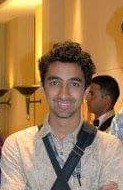
\includegraphics[width=1in,height=1.25in,clip,keepaspectratio]{sg}}]{Sulav Ghimire}
    received his intermediate degree in science from DAVSKVB, Jawalakhel, Nepal in 2013. He is currently a final year of student Undergraduate level of Electrical Engineering at Tribhuwan Unoversity, IOE Central Campus, Pulchowk. He has a good knowledge in power system simulation and also a winner of 2nd Inter College MATLAB simulation competition 2016. He has also won the first prize for case study competition organized by Locus-2016. His research field interests are power system stability, control system and photovoltaics.
\end{IEEEbiography}

\end{document}

